\appendix
\pagenumbering{Roman}
\thispagestyle{empty}  
\renewcommand{\appendixname}{Appendix}%%přílohy, číslování římskými


\chapter*{Appendix}
\addcontentsline{toc}{chapter}{Appendix}

\section{Technické detaily}

The device comunicates with brltty with the UOBP driver found at \footnote{\url{https://github.com/timthelion/UOBP}}.  The arduino is to be flashed with the FCHAD firmware found at the same url.  The arduino is connected to 8 paralel solenoid circuites as described here \footnote{\url{http://playground.arduino.cc/uploads/Learning/solenoid_driver.pdf}}, using MOSFETs of type IRF530N.  The solenoid power circute is powered by a 6 volt 4 amp wall power supply of type "Smart Electronic Switching adapter Model:JGS1002-24060-2E".  Touches were detected using a 16 channel MUX of type CMOS4067 connected to 4 digital IO pins and one analog pin.  The analog pin was connected to ground with a 10k ohm resistor of type RM0207 "resistor with metalic layer 1\% TK50 0.5W RM 7.5mm".


\clearpage
\begin{figure}
\section{Obrazky FCHADu}
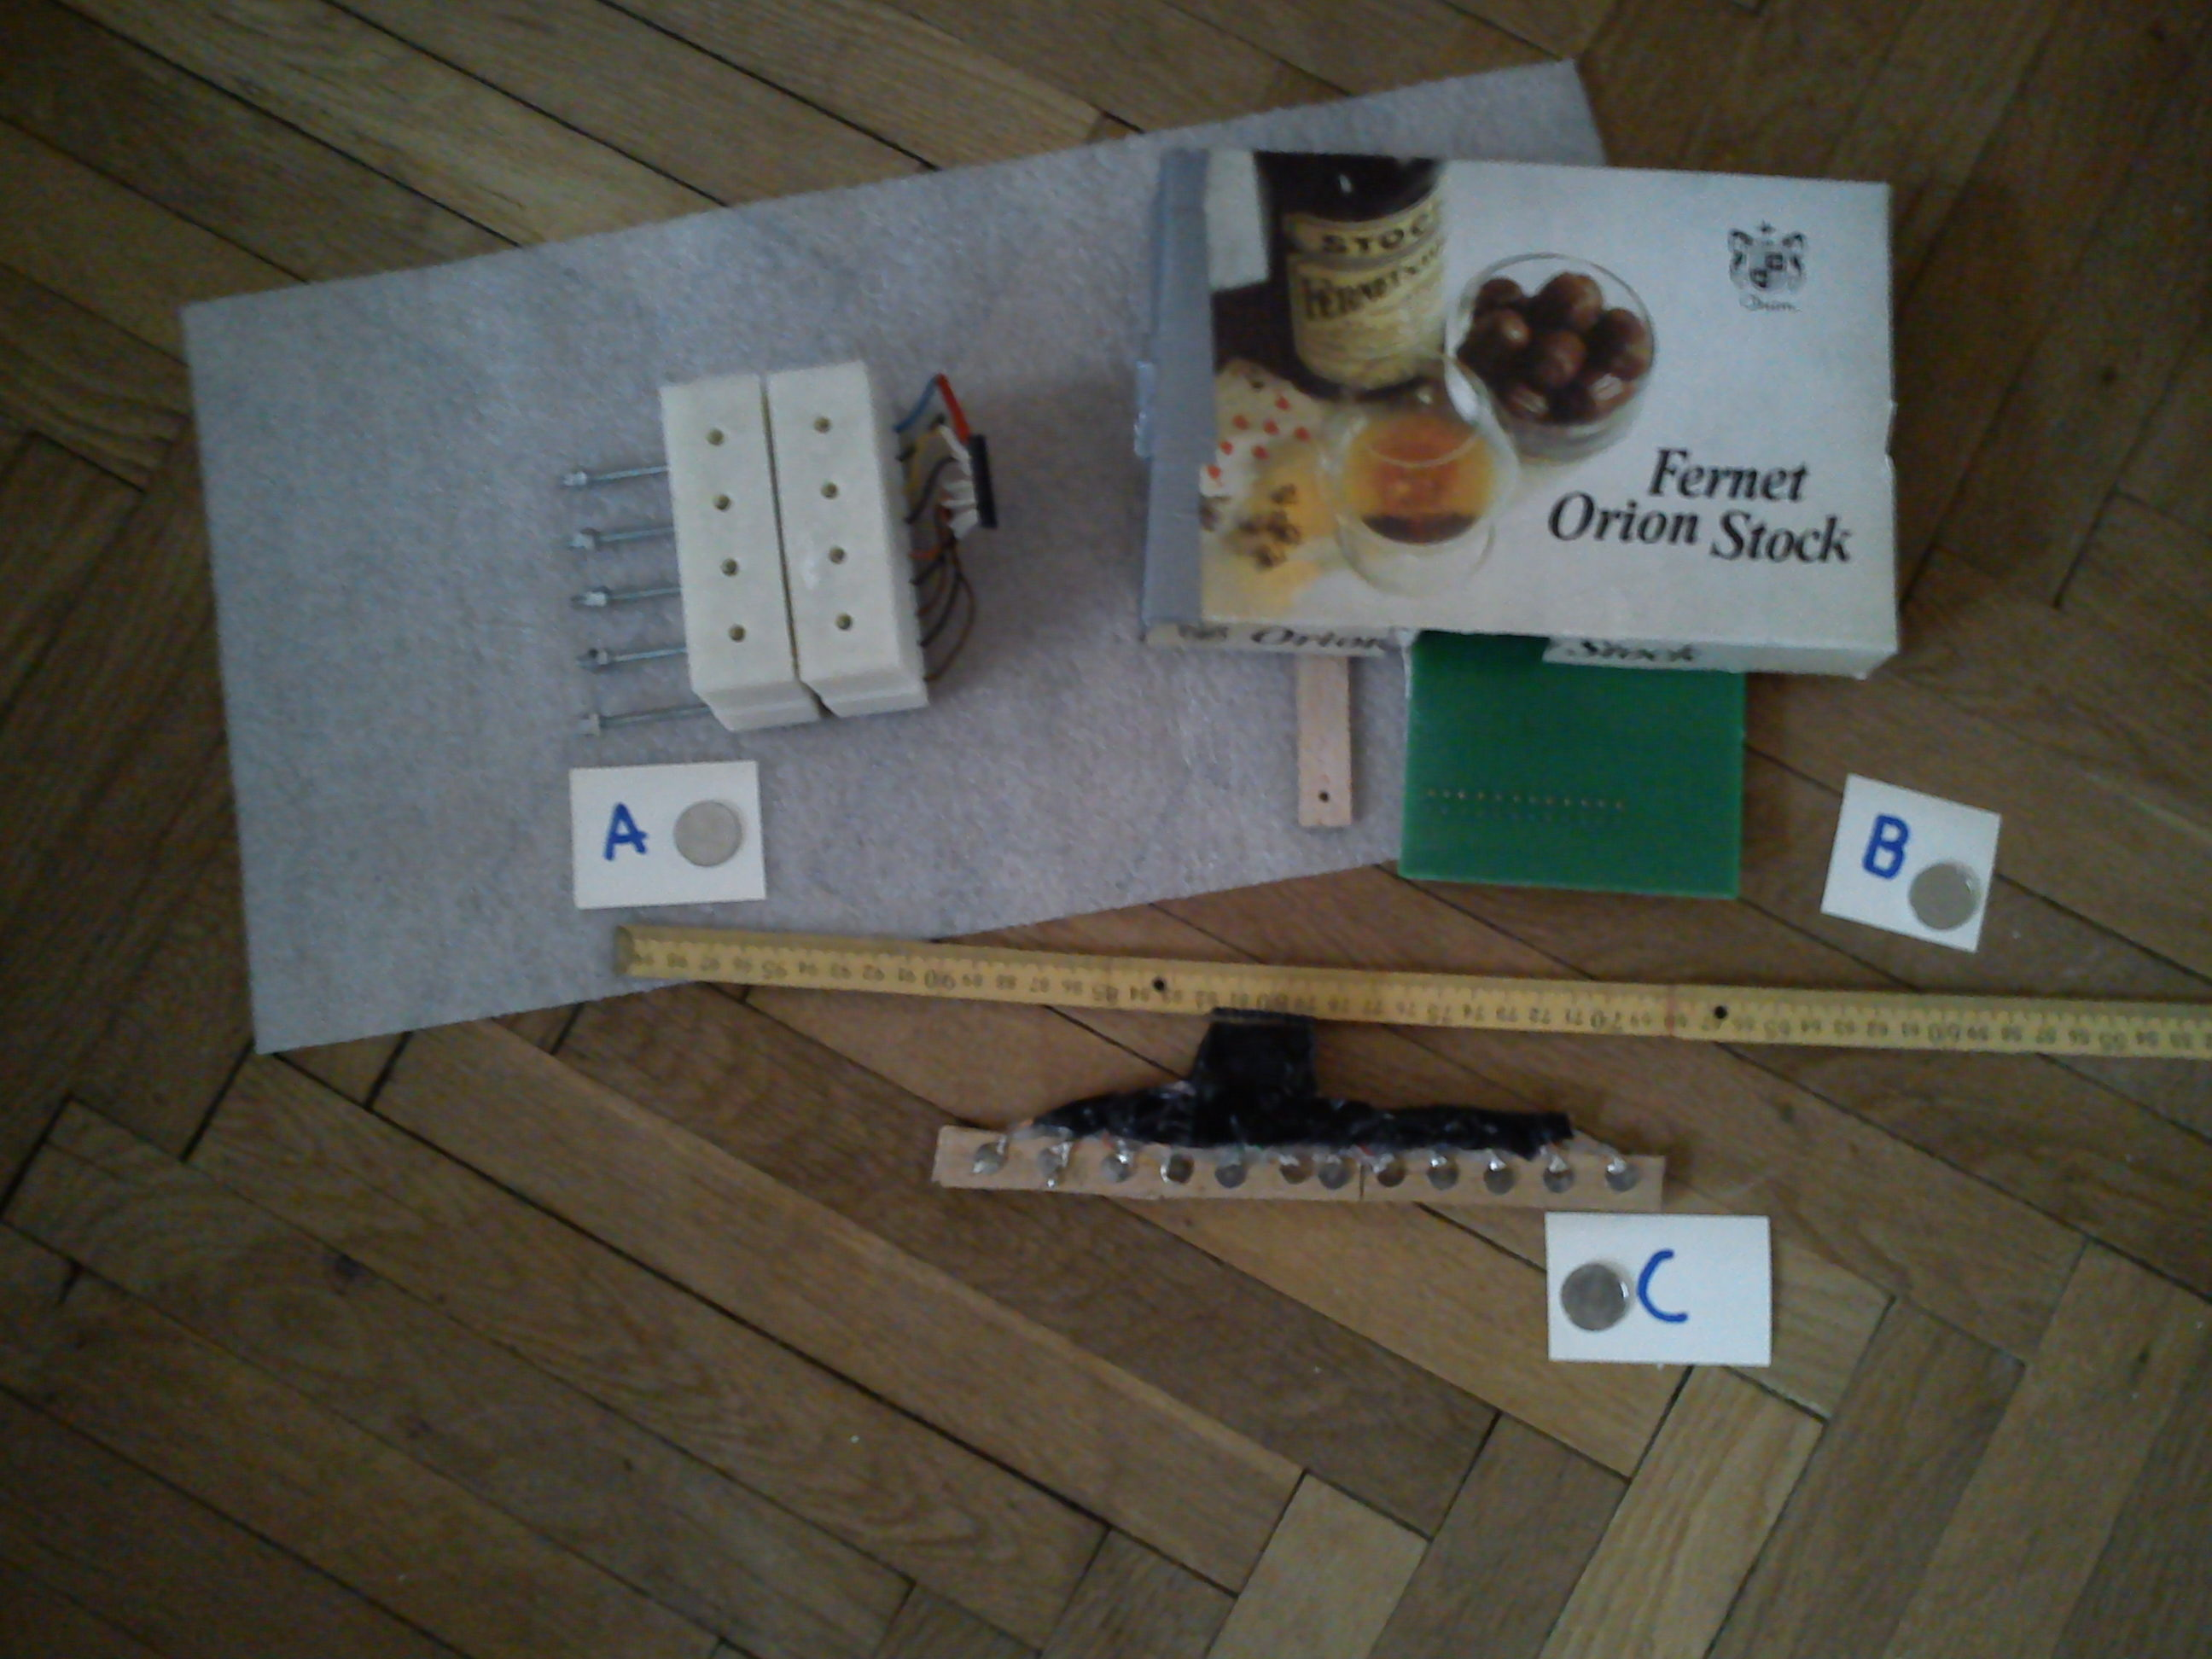
\includegraphics[width=1\textwidth]{Device1}
\begin{subfigure}{.5\textwidth}
  \centering
  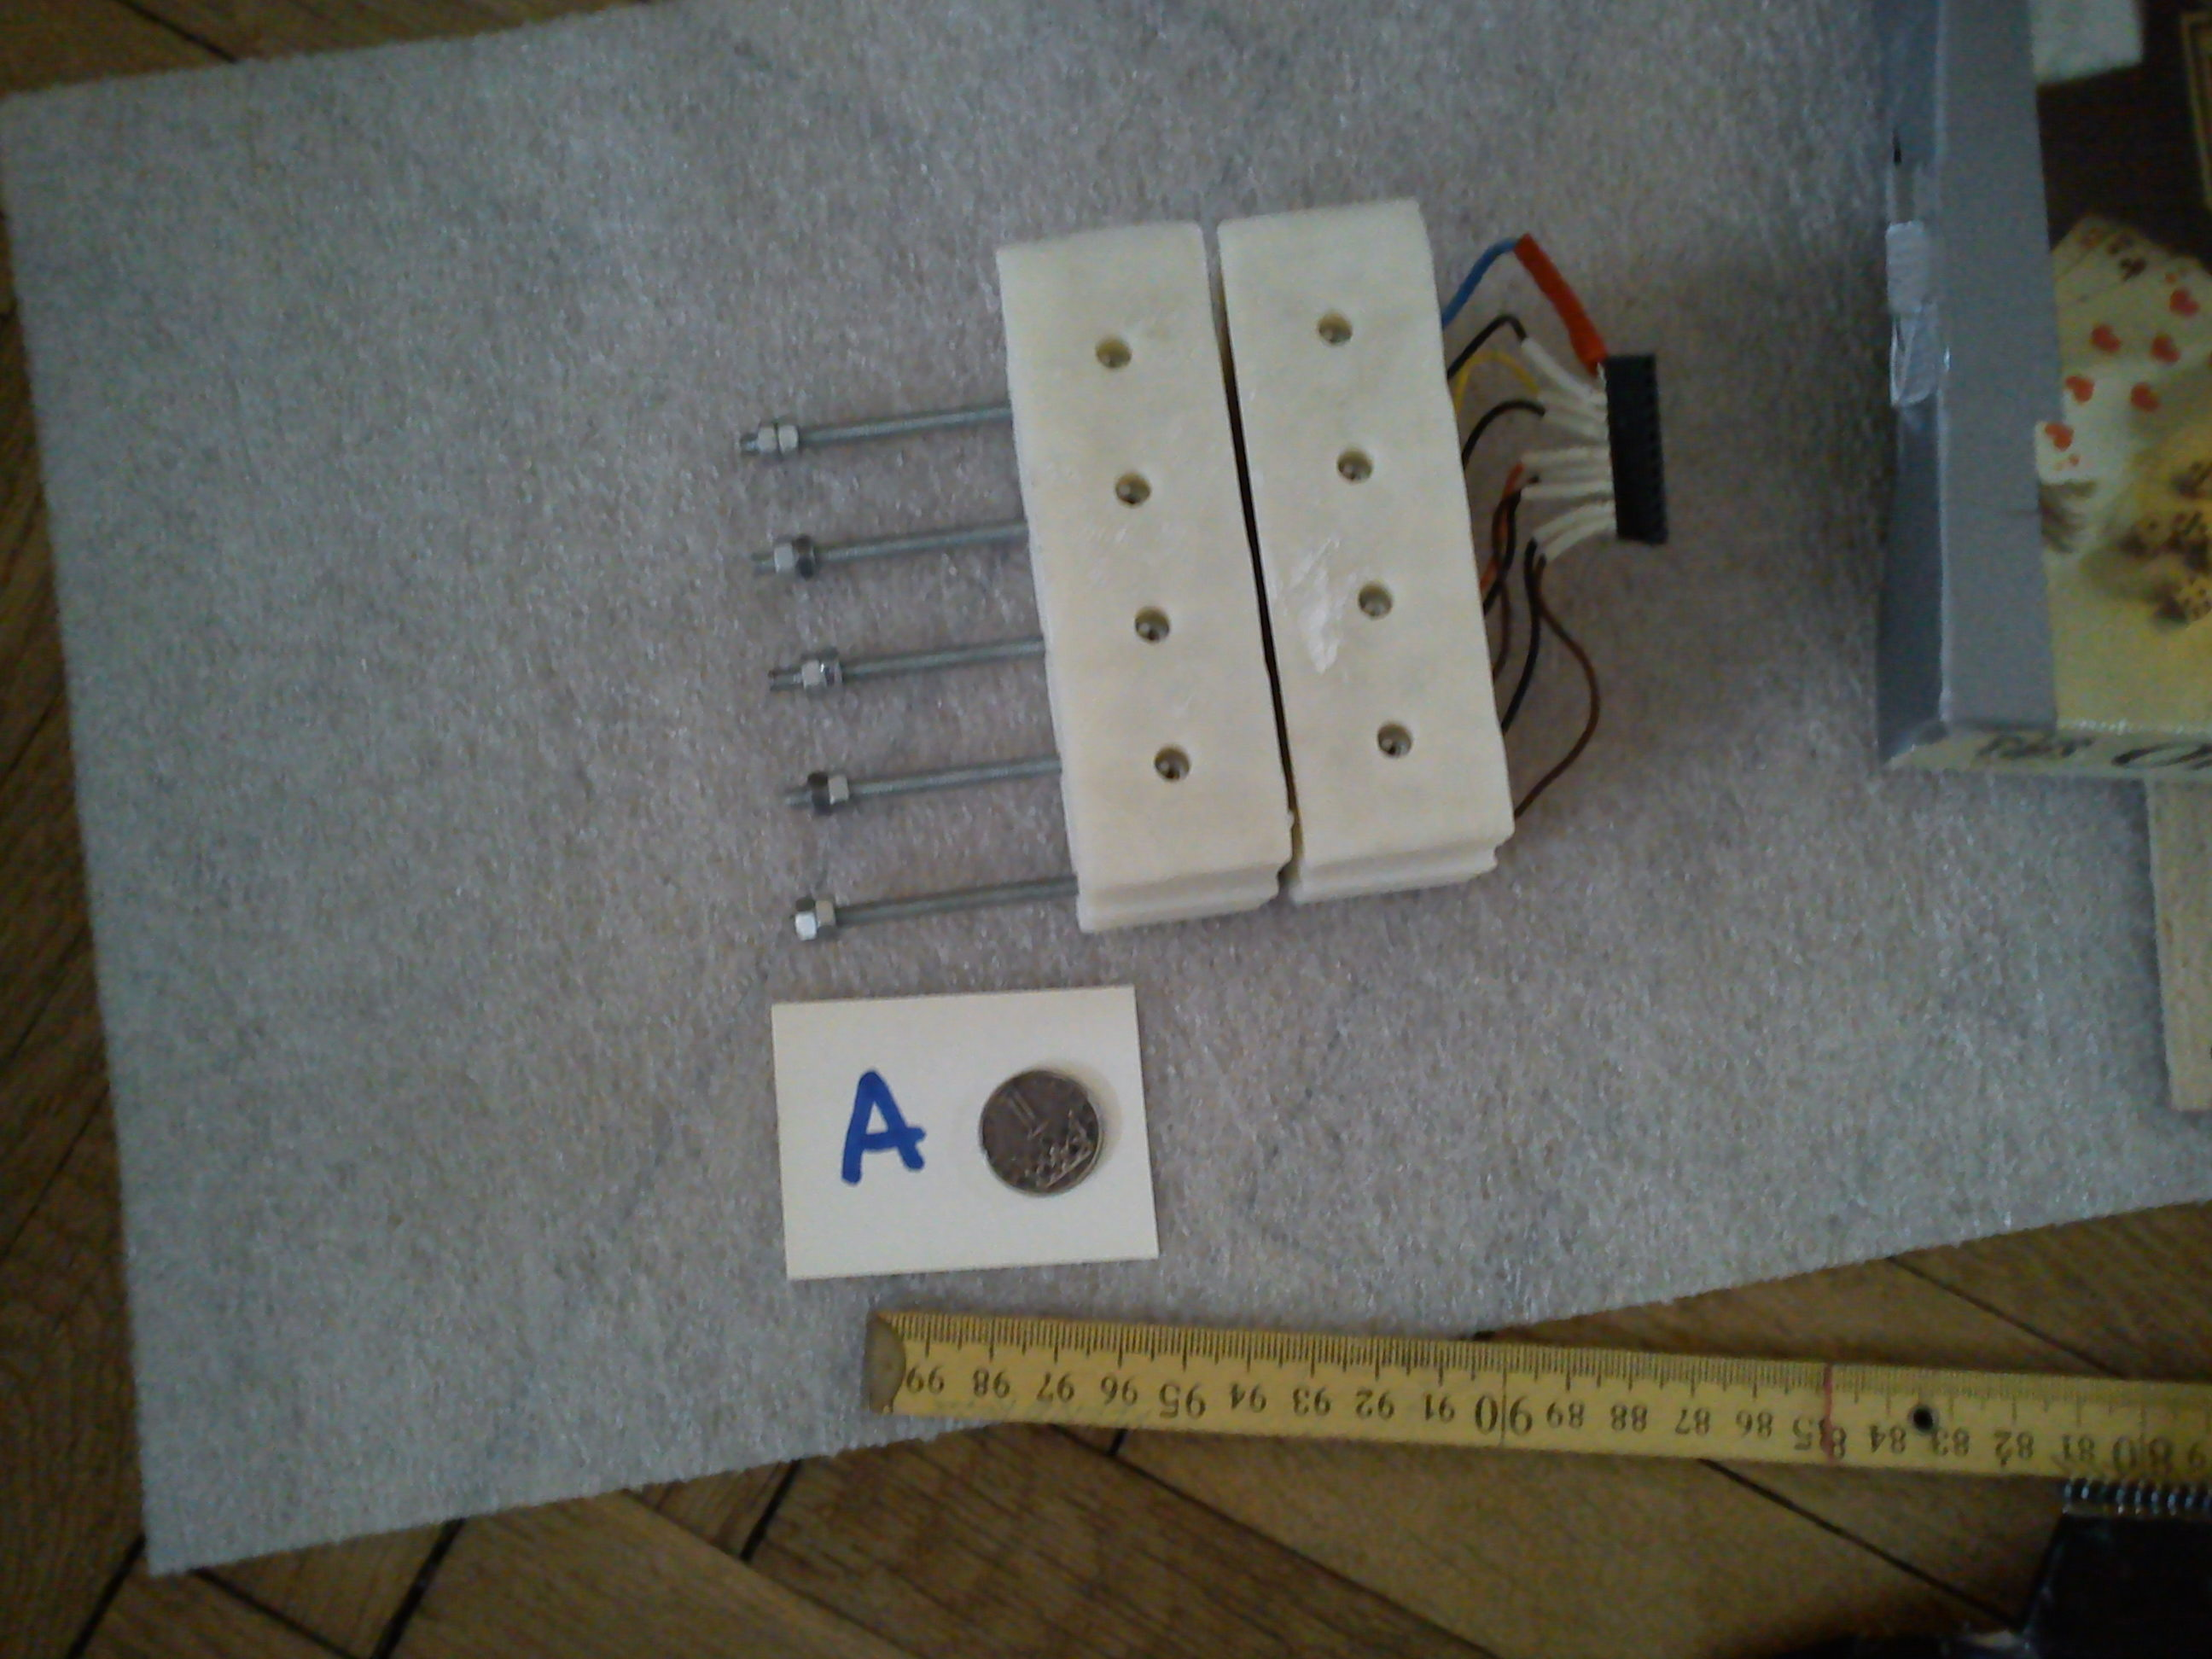
\includegraphics[width=.95\linewidth]{Device1-A}
  \caption{Obrazek 1-A - Zobrazovač}
  \label{fig:sub1}
\end{subfigure}%
\begin{subfigure}{.5\textwidth}
  \centering
  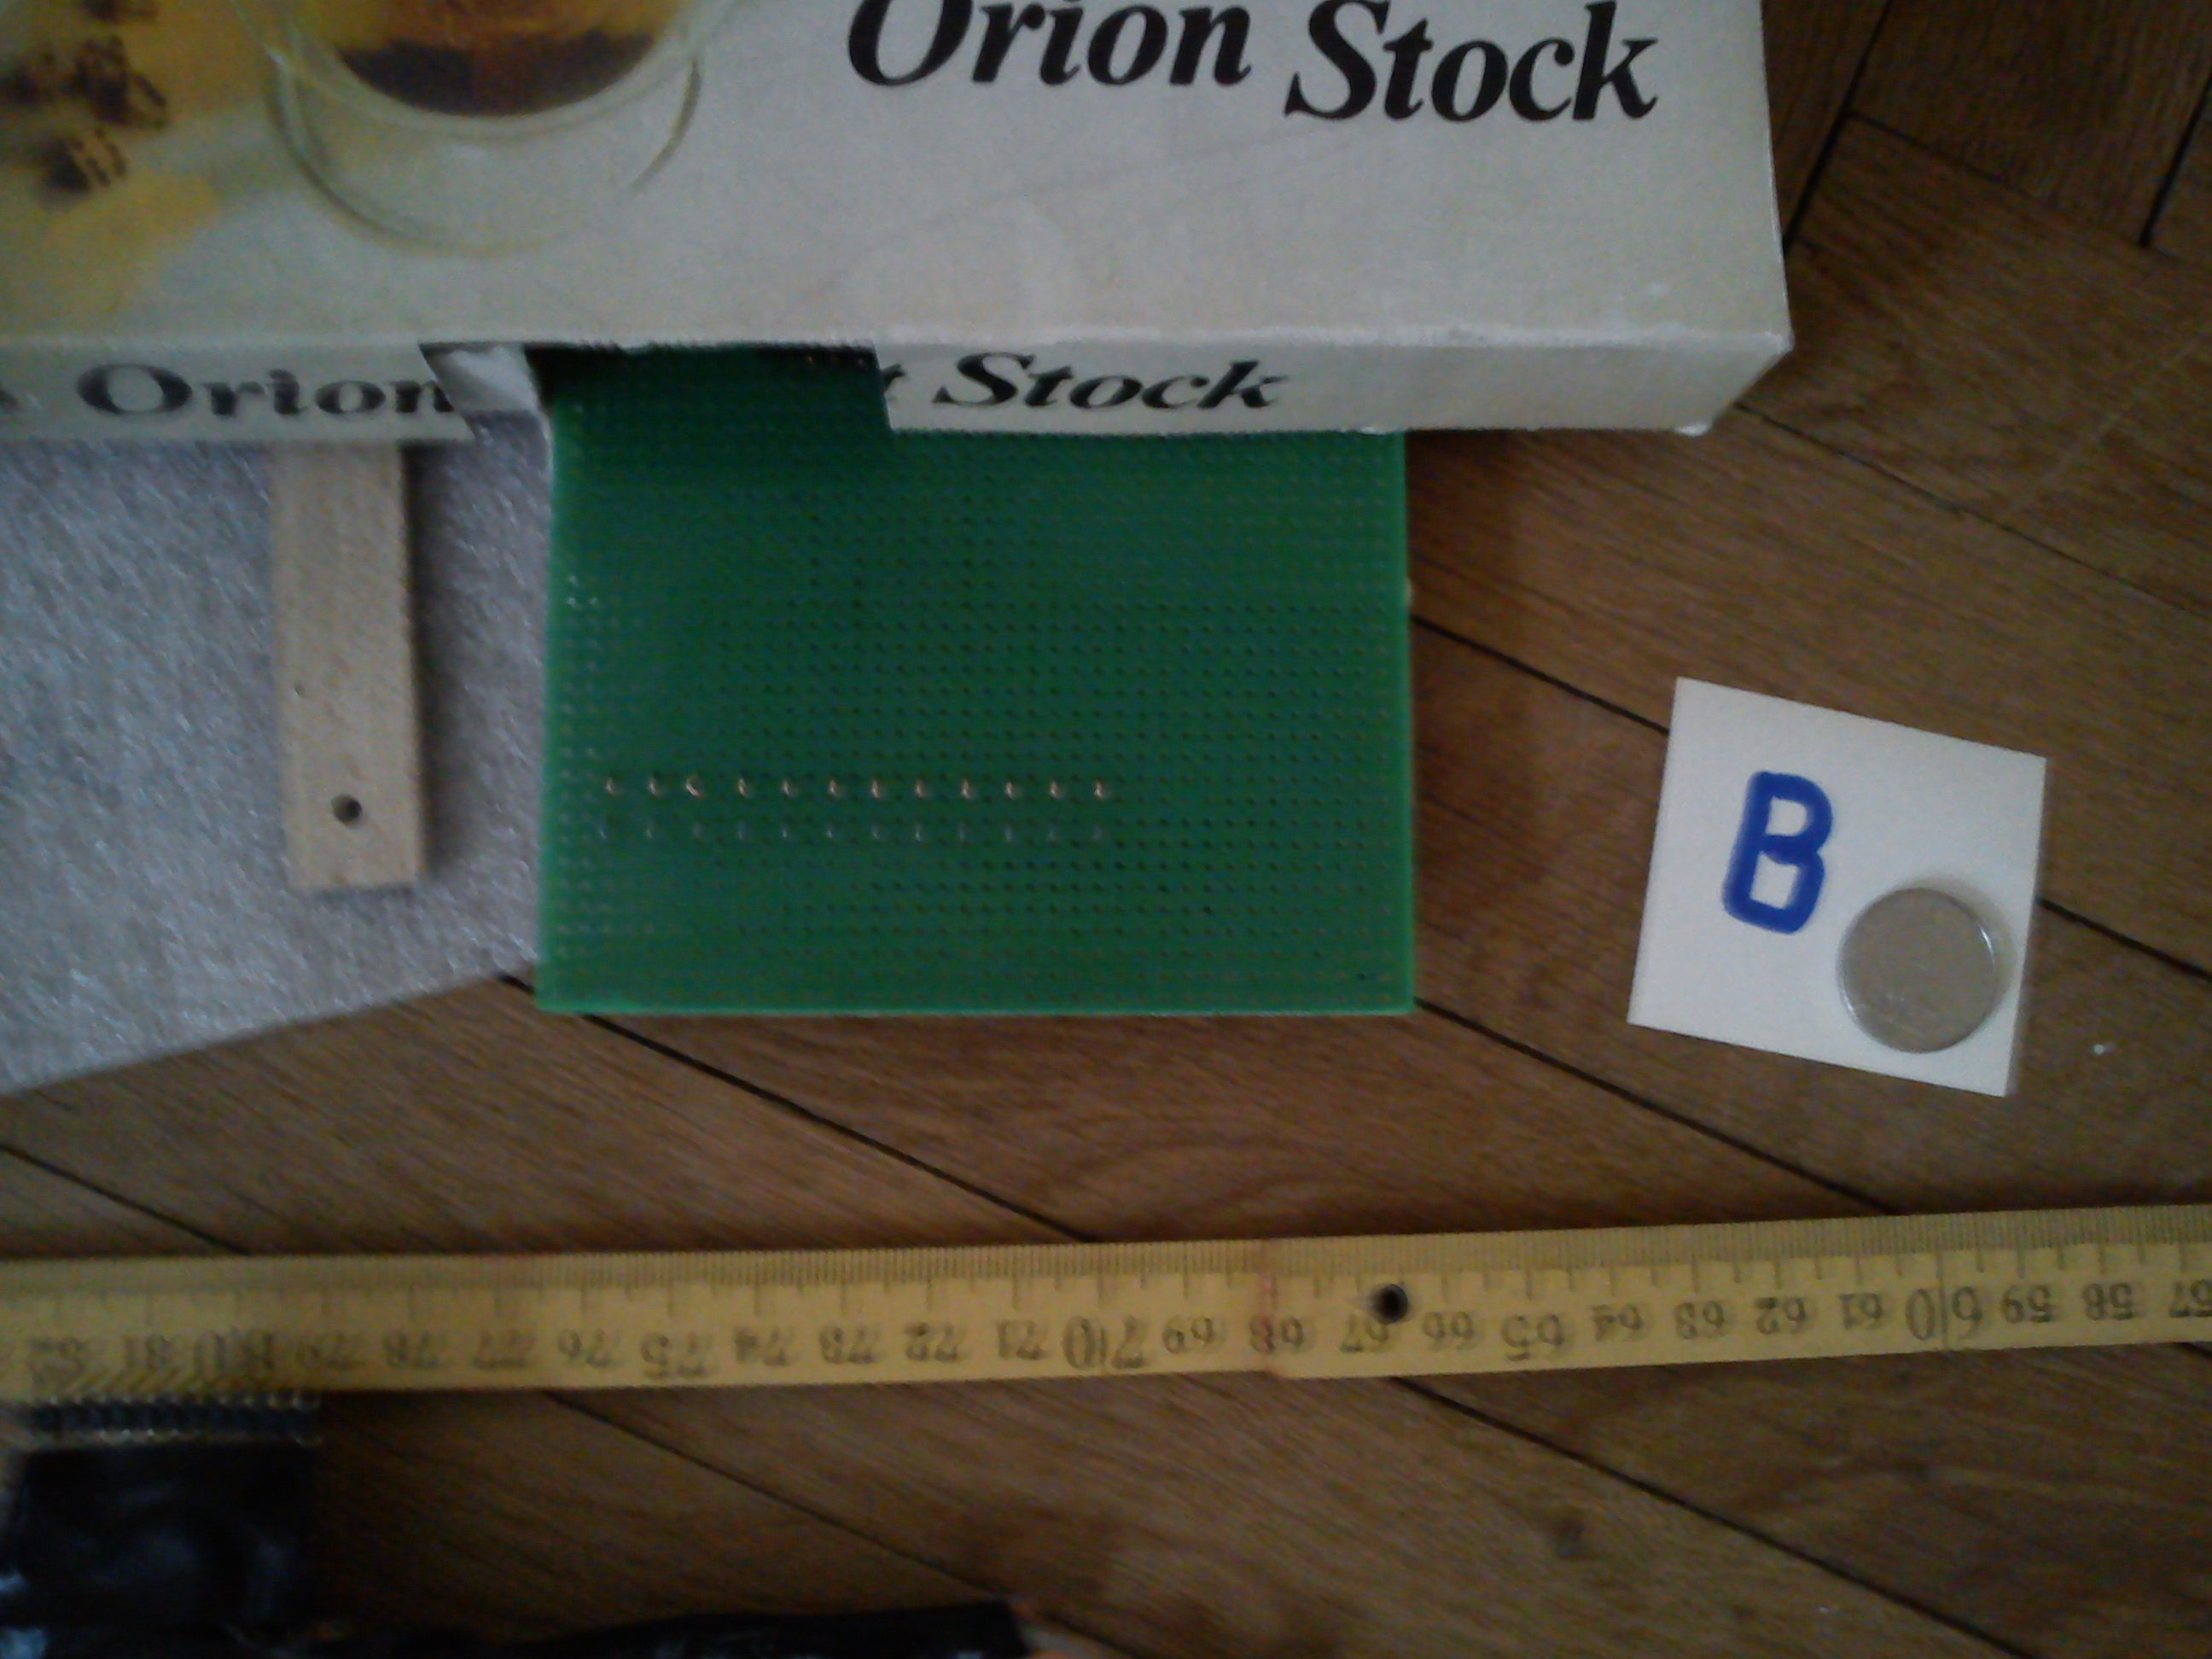
\includegraphics[width=.95\linewidth]{Device1-B}
  \caption{Obrazek 1-B - Kursor selektor}
  \label{fig:sub2}
\end{subfigure}

\label{fig:test}
\end{figure}
\begin{figure}
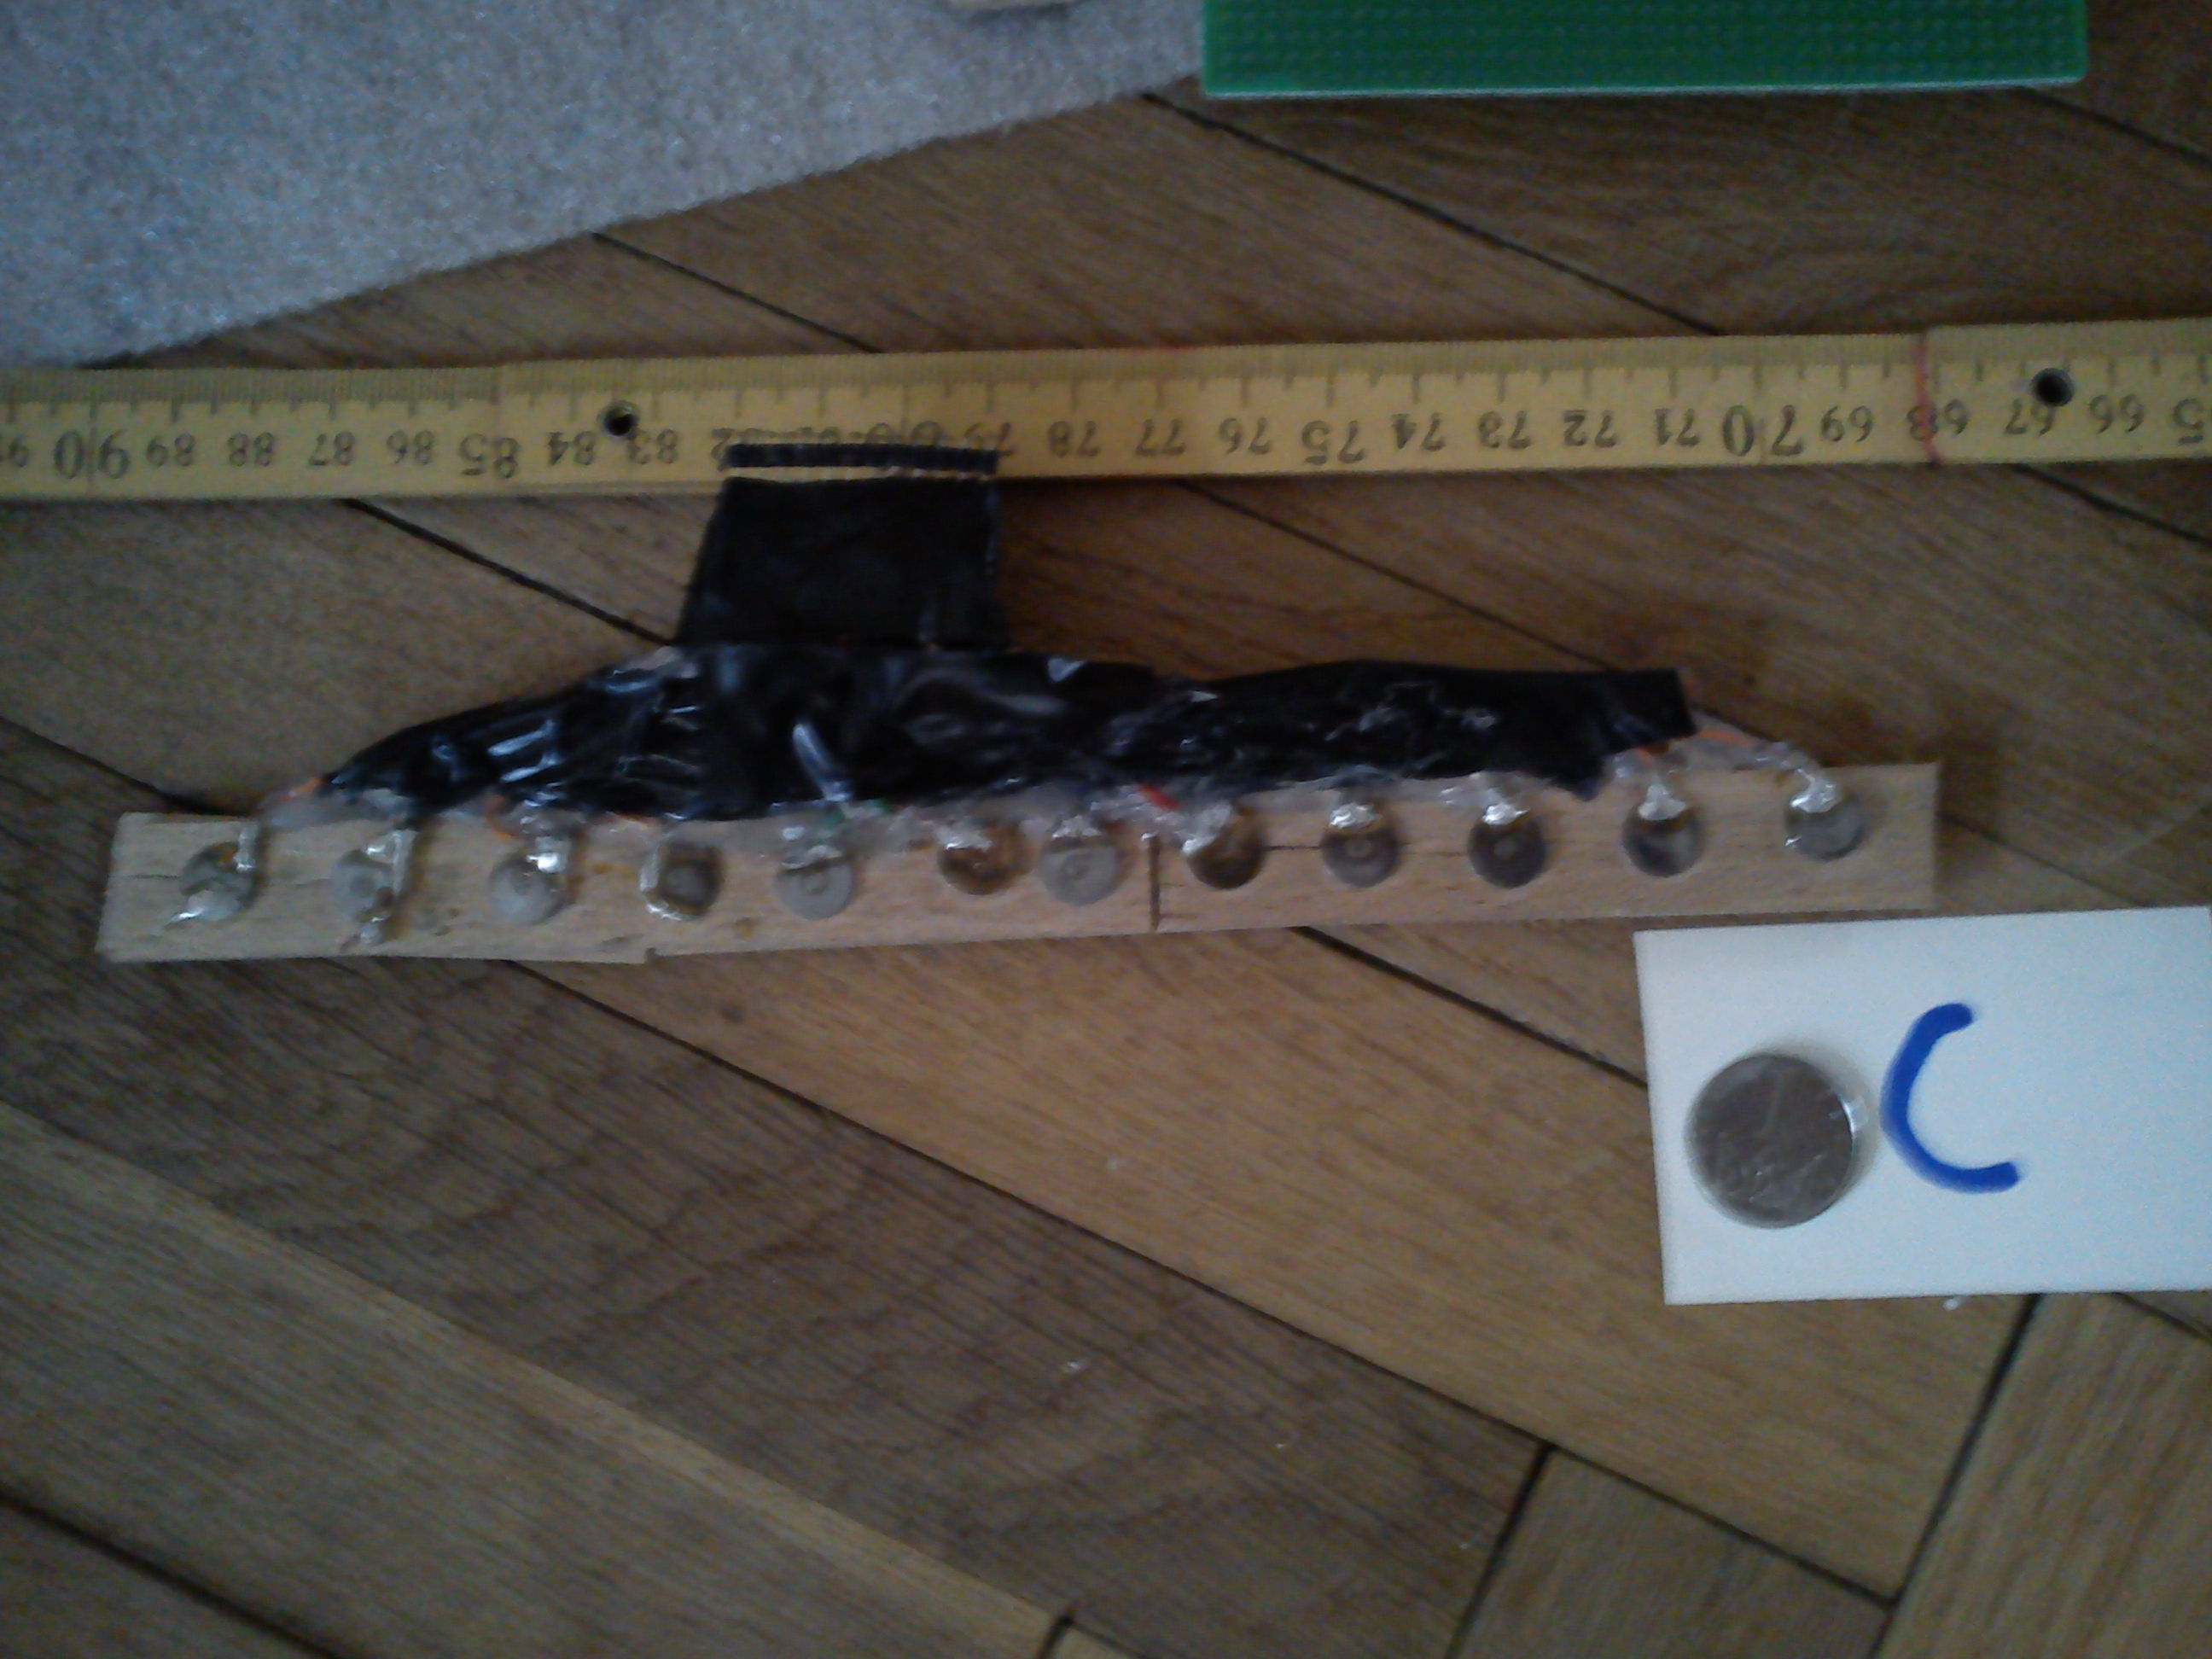
\includegraphics[width=.7\linewidth]{Device1-C}
\caption{Obrazek 1-C - Starý kursor selektor}
\label{fig:sub2}
\end{figure}

\begin{figure}
\centering
\begin{subfigure}{.5\textwidth}
  \centering
  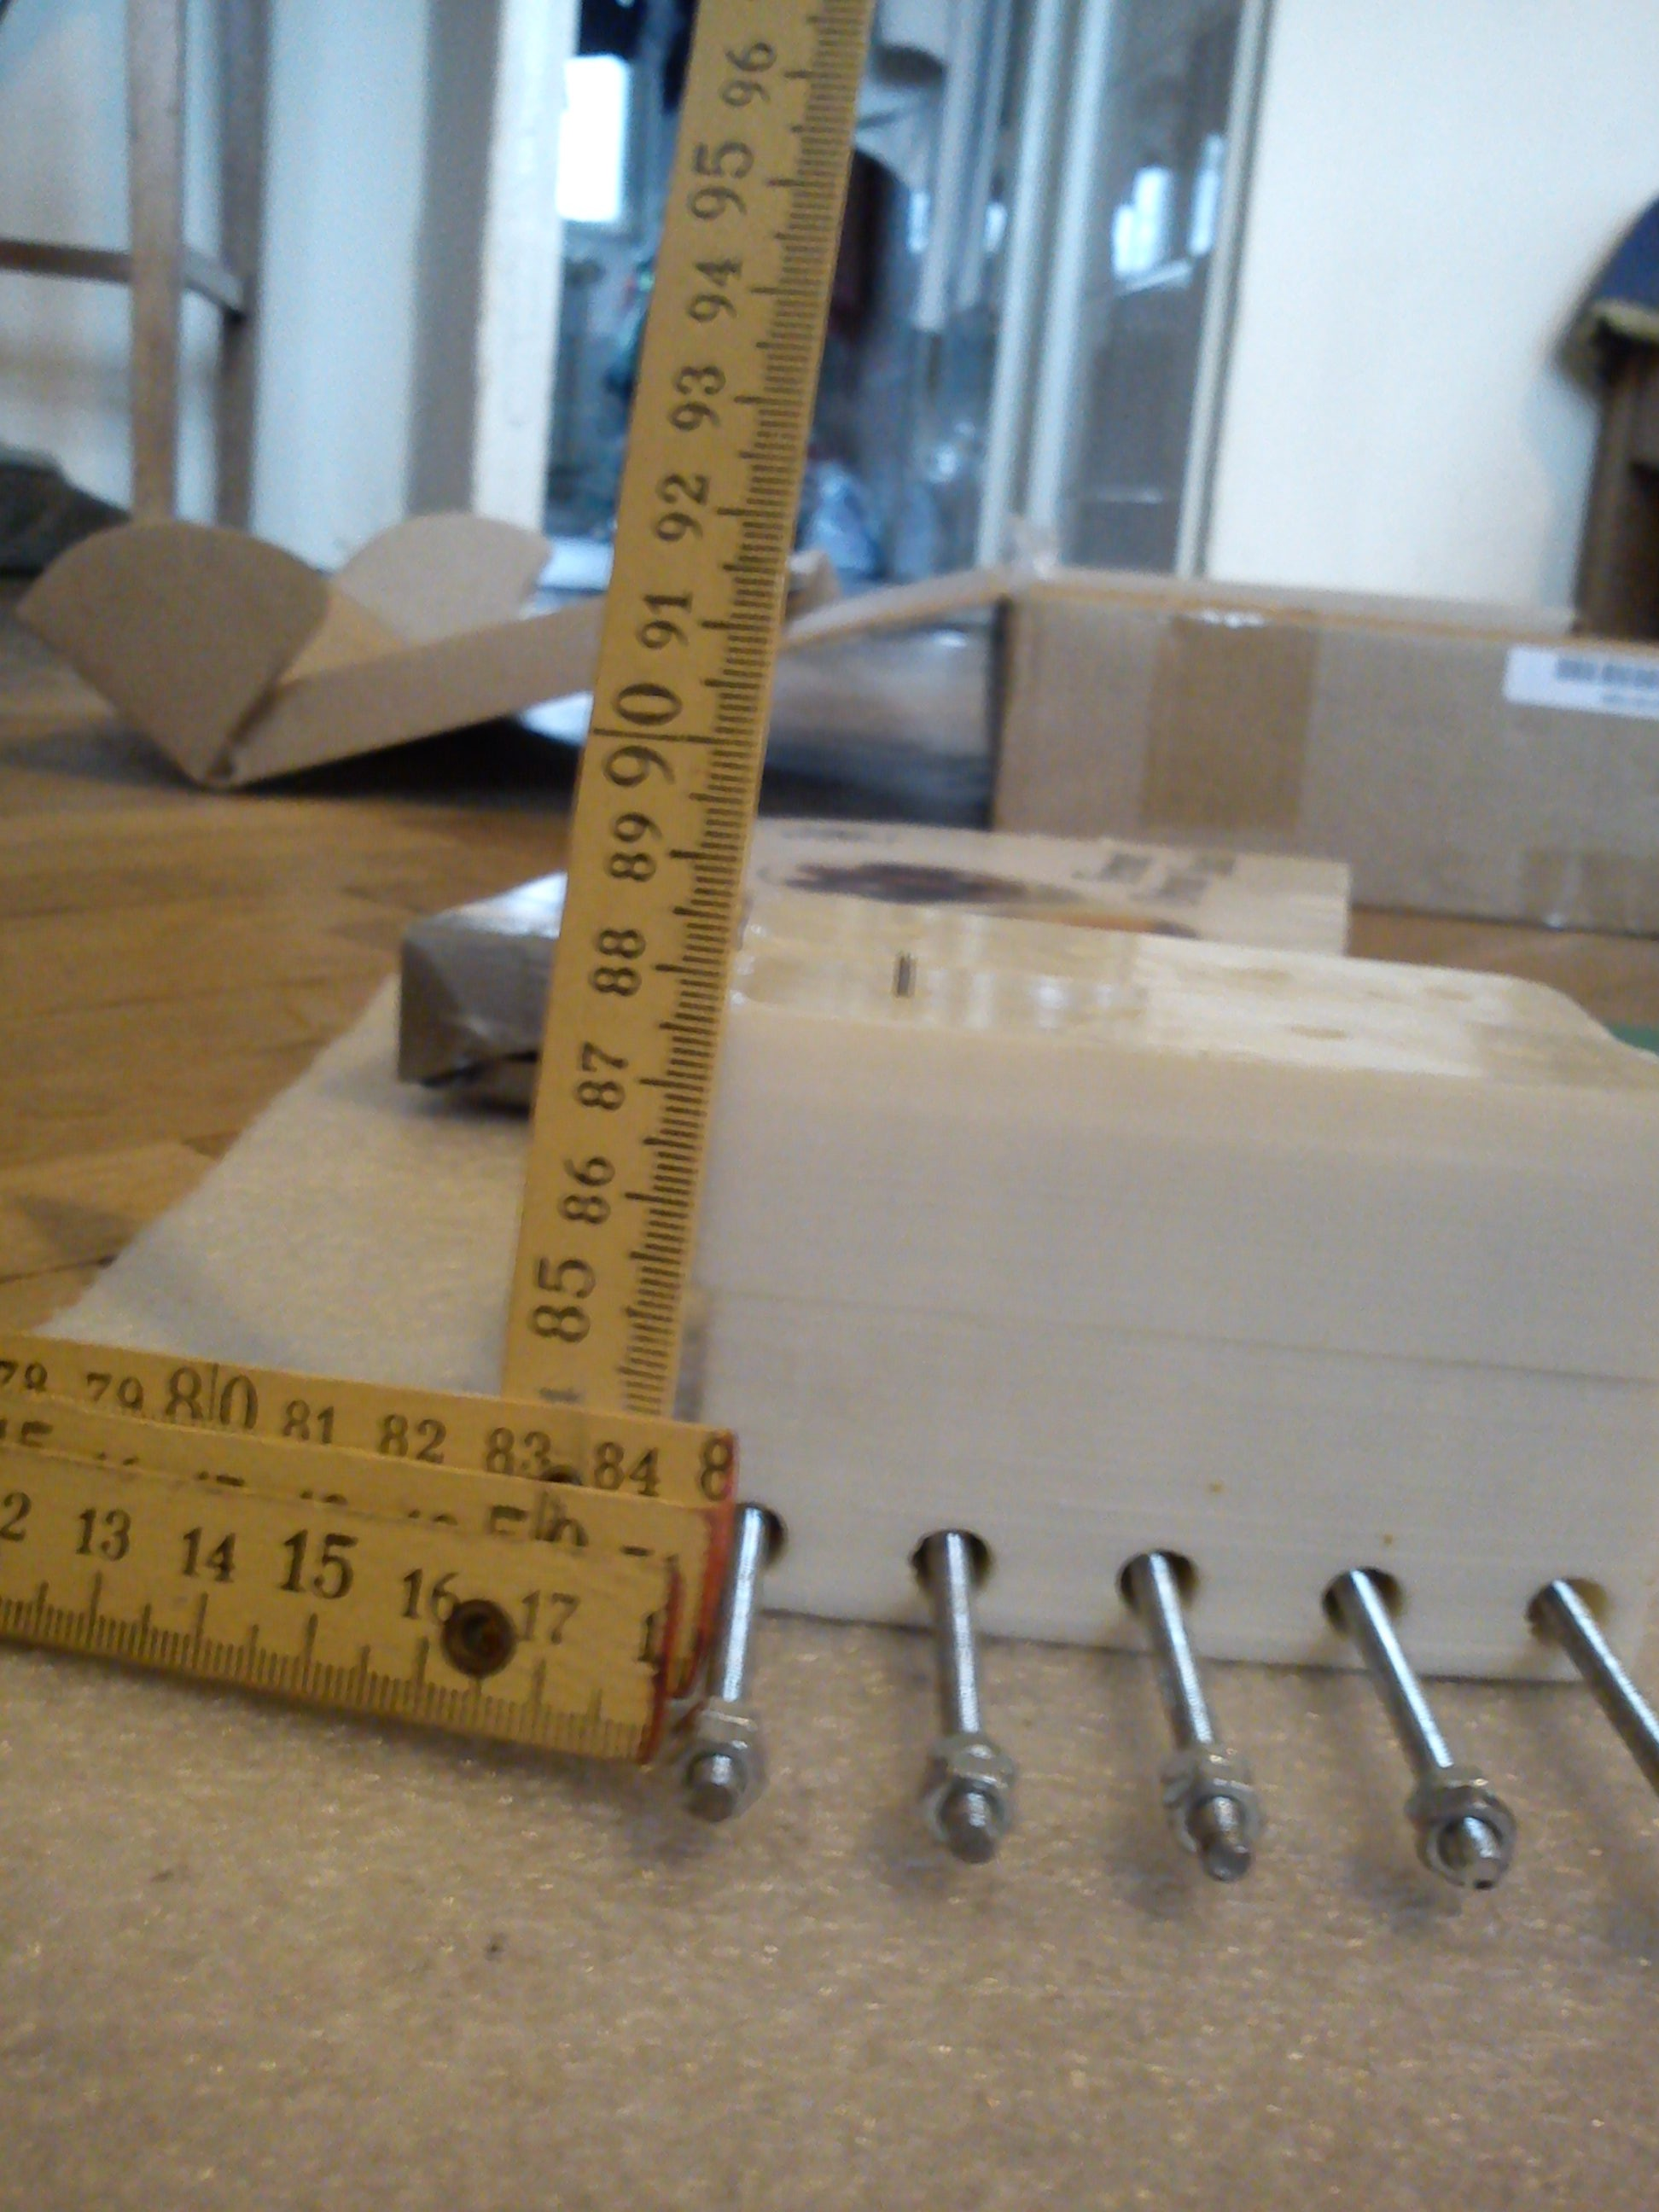
\includegraphics[width=.8\linewidth]{Device2}
  \caption{Obrazek 2 - Zobrazovač ze strany}
  \label{fig:sub1}
\end{subfigure}%
\begin{subfigure}{.5\textwidth}
  \centering
  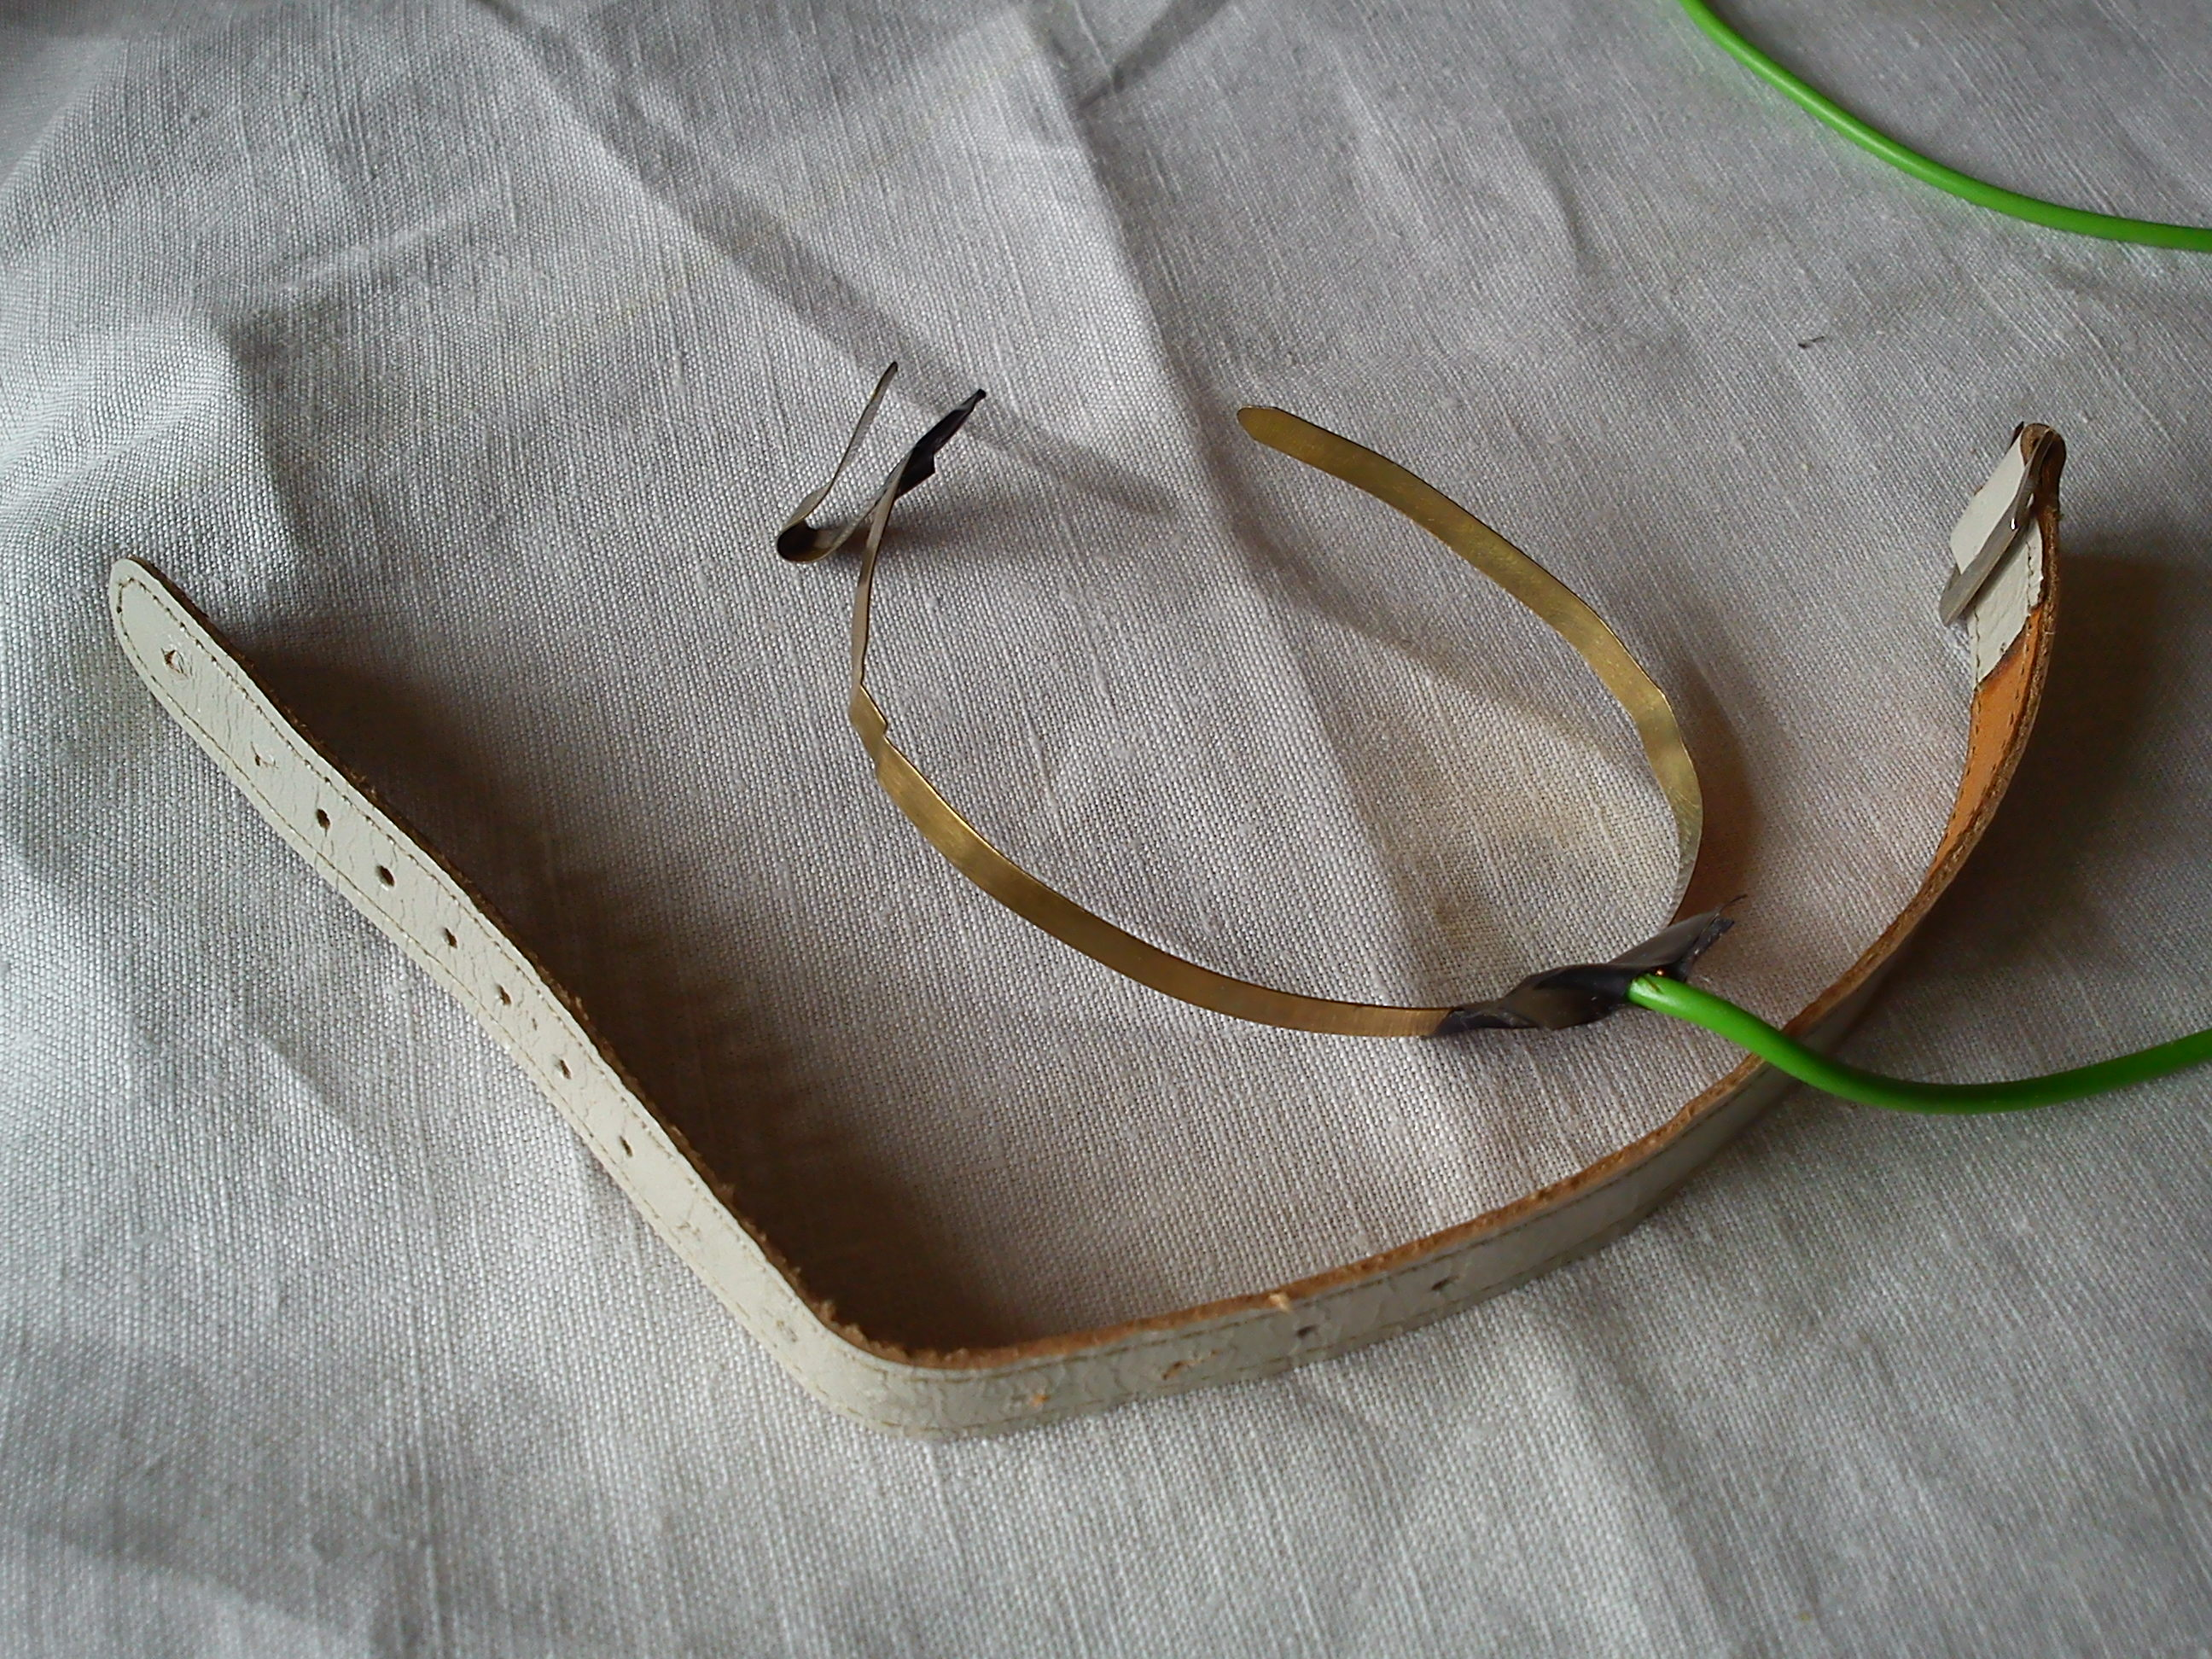
\includegraphics[width=.8\linewidth]{Device3}
  \caption{Obrazek 3 - Zapesní elektrod}
  \label{fig:sub2}
\end{subfigure}
\label{fig:test}
\end{figure}
\clearpage

%\center
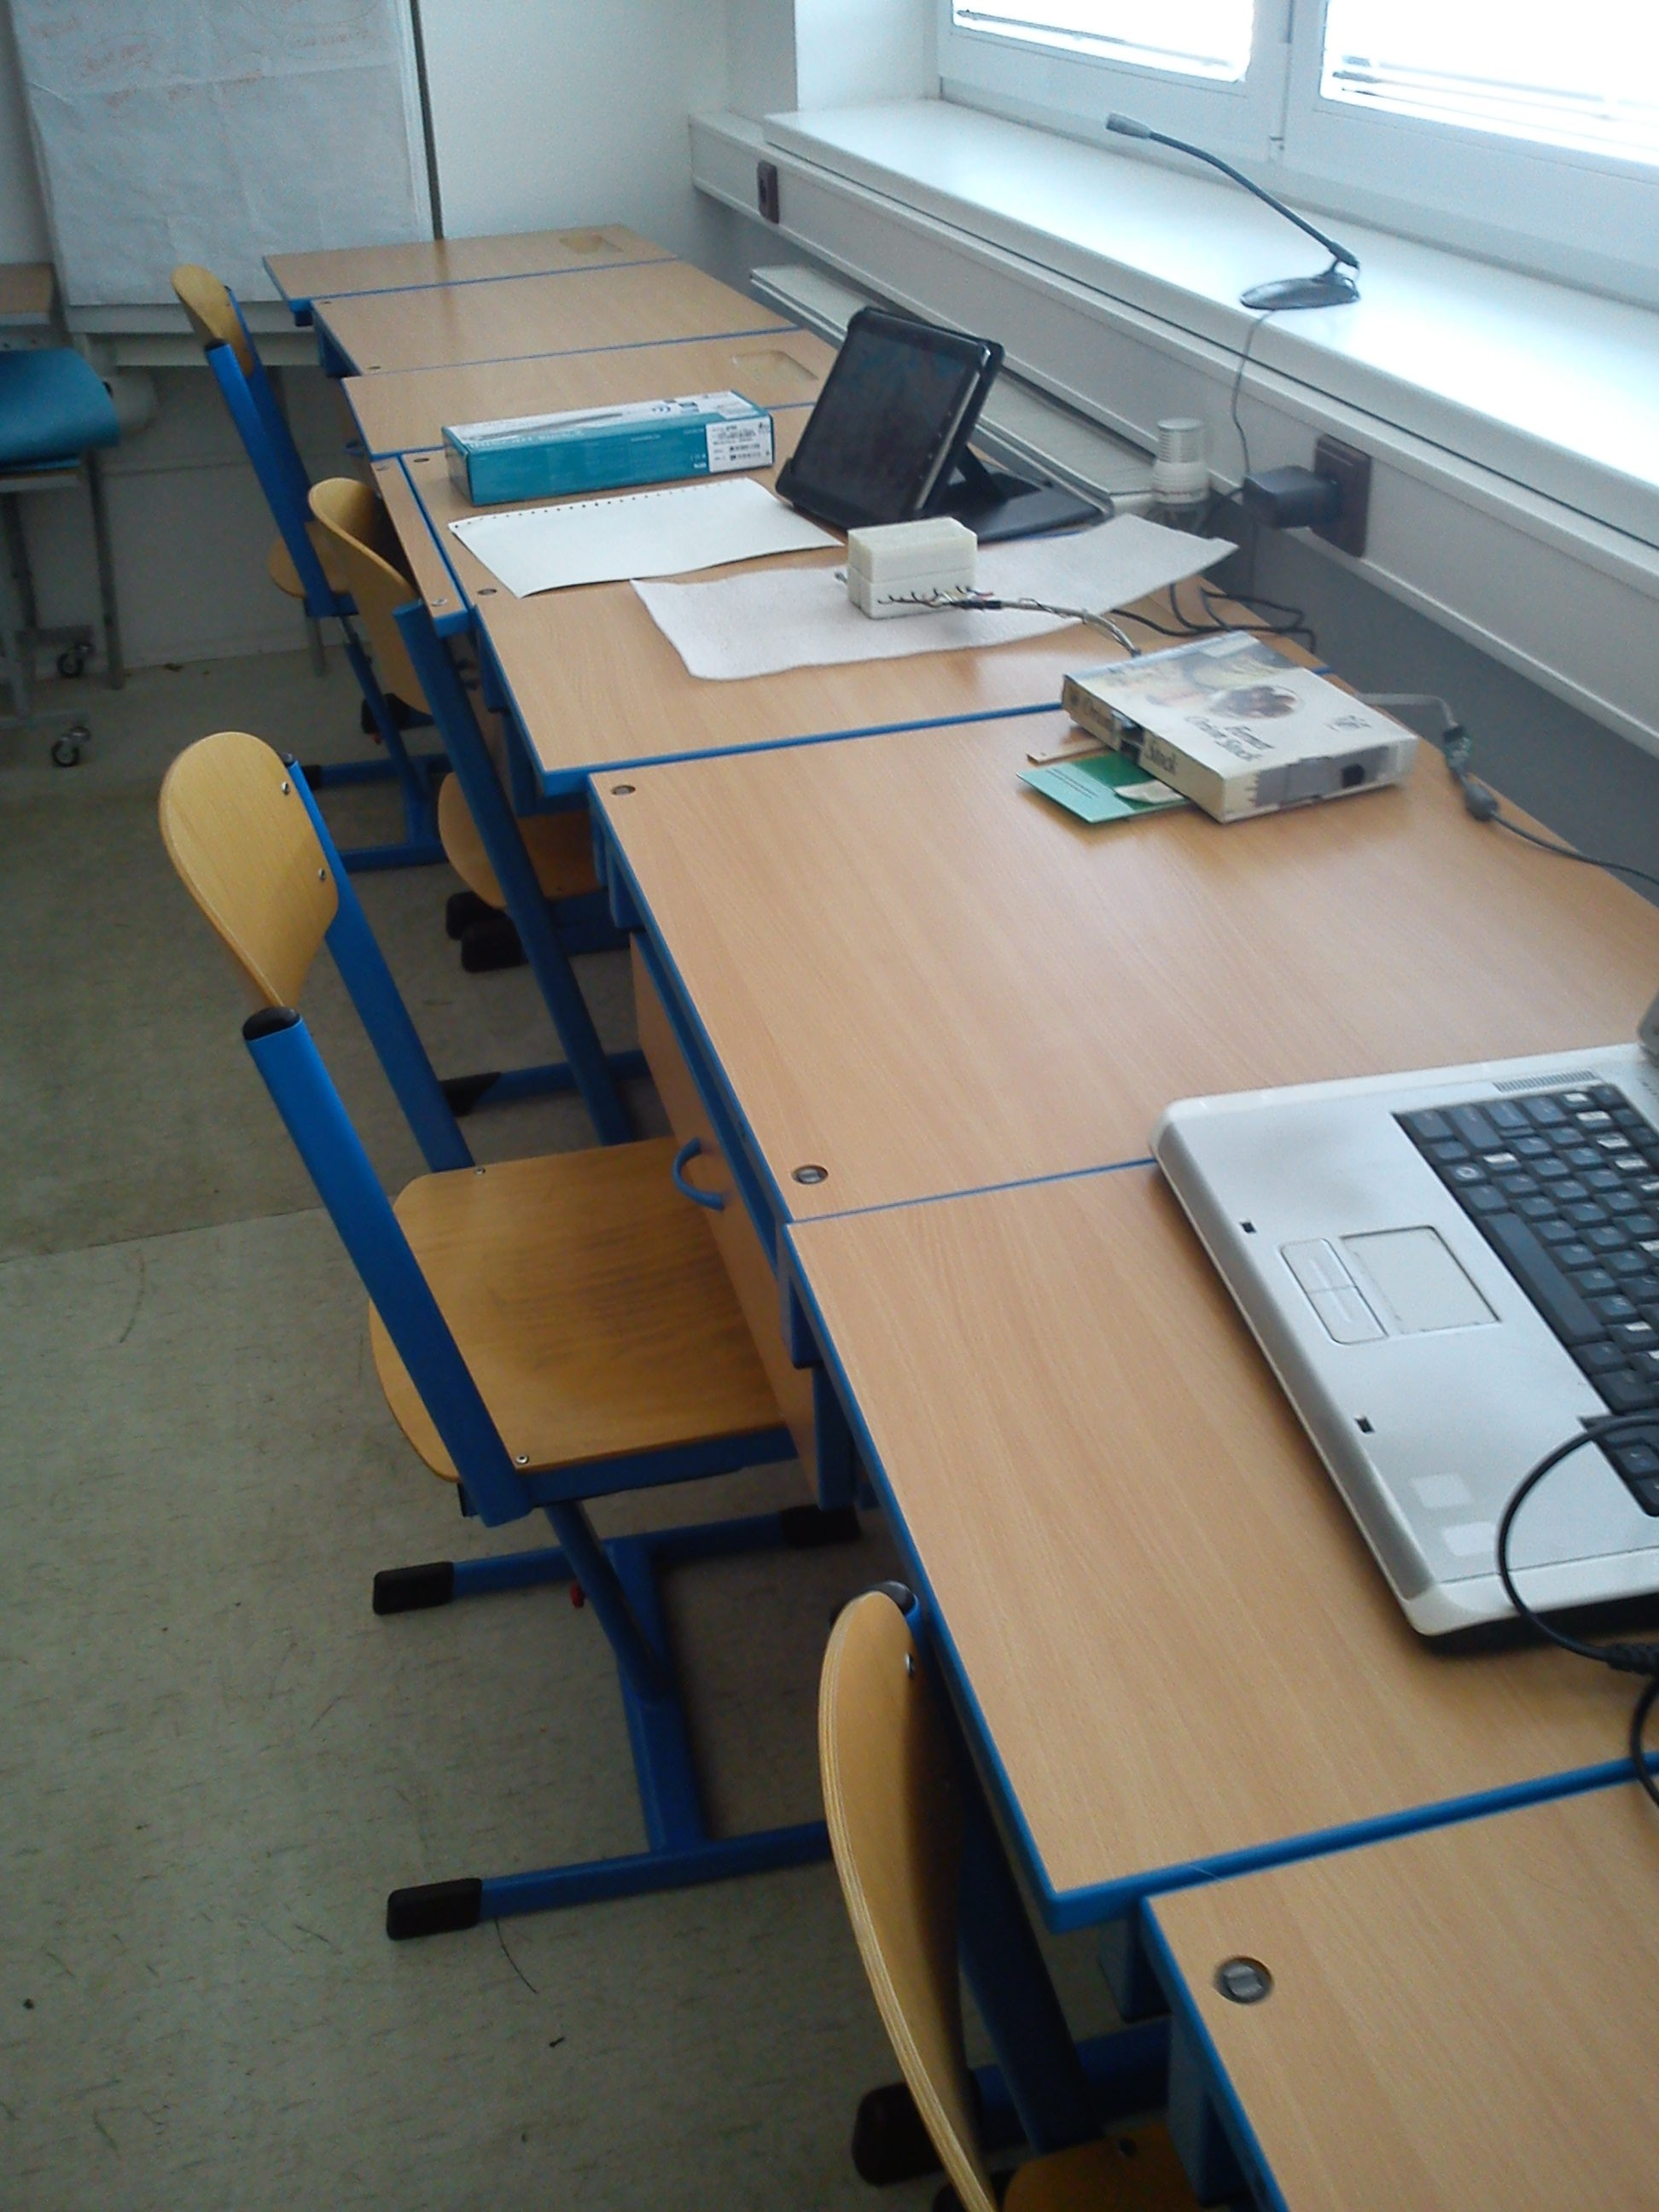
\includegraphics[width=.9\textwidth]{Gymnasium}

Obrazek 4 - Místo konání běžného studia
%\endcenter

\clearpage

\section{Text na FCHAD}

Tady je čast textu, který dočetl nejlepší čtenář s braillským překladem.

%\paragraph{První Řádek}
\begin{tabular}{|c|c|c|c|c|c|c|c|c|c|c|c|}
\hline
B&r&a&i&l&l&s&&&&&\\
\braillebox{1278}&\braillebox{1235}&\braillebox{1}&\braillebox{24}&\braillebox{123}&\braillebox{123}&\braillebox{234}&\braillebox{}&\braillebox{2358}&\braillebox{123}&\braillebox{}&\braillebox{}\\
\hline
\end{tabular}

%\paragraph{Druhý Řádek}
\begin{tabular}{|c|c|c|c|c|c|c|c|c|c|c|c|}
\hline
k&ý& &ř&á&d&e&k&,& &k&t\\
\braillebox{1378}&\braillebox{12346}&\braillebox{}&\braillebox{2456}&\braillebox{16}&\braillebox{145}&\braillebox{15}&\braillebox{13}&\braillebox{2}&\braillebox{}&\braillebox{13}&\braillebox{2345}\\
\hline
\end{tabular}

%\paragraph{Třetí Řádek}
\begin{tabular}{|c|c|c|c|c|c|c|c|c|c|c|c|}
\hline
e&r&ý& &t&e&ď& &p&o&u&ž\\
\braillebox{1578}&\braillebox{1235}&\braillebox{12346}&\braillebox{}&\braillebox{2345}&\braillebox{15}&\braillebox{1456}&\braillebox{}&\braillebox{1234}&\braillebox{135}&\braillebox{136}&\braillebox{2346}\\
\hline
\end{tabular}

%\paragraph{Čtvrtý Řádek}
\begin{tabular}{|c|c|c|c|c|c|c|c|c|c|c|c|}
\hline
í&v&á&t&e&,& &n&e&n&í& \\
\braillebox{3478}&\braillebox{1236}&\braillebox{16}&\braillebox{2345}&\braillebox{15}&\braillebox{2}&\braillebox{}&\braillebox{1345}&\braillebox{15}&\braillebox{1345}&\braillebox{34}&\braillebox{}\\
\hline
\end{tabular}

%\paragraph{Pátý Řádek}
\begin{tabular}{|c|c|c|c|c|c|c|c|c|c|c|c|}
\hline
p&r&v&n&í& &ř&á&d&e&k&,\\
\braillebox{123478}&\braillebox{1235}&\braillebox{1236}&\braillebox{1345}&\braillebox{34}&\braillebox{}&\braillebox{1235}&\braillebox{16}&\braillebox{145}&\braillebox{15}&\braillebox{13}&\braillebox{2}\\
\hline
\end{tabular}

%\paragraph{Šestý Řádek}
\begin{tabular}{|c|c|c|c|c|c|c|c|c|c|c|c|}
\hline
 &k&t&e&r&ý& &z&o&b&r&a\\
\braillebox{78}&\braillebox{13}&\braillebox{2345}&\braillebox{15}&\braillebox{1235}&\braillebox{12346}&\braillebox{}&\braillebox{1356}&\braillebox{135}&\braillebox{12}&\braillebox{1235}&\braillebox{1}\\
\hline
\end{tabular}

%\paragraph{Řádek 7}
\begin{tabular}{|c|c|c|c|c|c|c|c|c|c|c|c|}
\hline
z&u&j&e& &j&e&n&o&m& &j\\
\braillebox{135678}&\braillebox{136}&\braillebox{245}&\braillebox{15}&\braillebox{}&\braillebox{245}&\braillebox{15}&\braillebox{1345}&\braillebox{135}&\braillebox{134}&\braillebox{}&\braillebox{245}\\
\hline
\end{tabular}

%\paragraph{Řádek 8}
\begin{tabular}{|c|c|c|c|c|c|c|c|c|c|c|c|}
\hline
e&d&n&o& &p&í&s&m&e&n&o\\
\braillebox{1578}&\braillebox{145}&\braillebox{1345}&\braillebox{135}&\braillebox{}&\braillebox{1234}&\braillebox{34}&\braillebox{234}&\braillebox{134}&\braillebox{15}&\braillebox{1345}&\braillebox{135}\\
\hline
\end{tabular}

%\paragraph{Řádek 9}
\begin{tabular}{|c|c|c|c|c|c|c|c|c|c|c|c|}
\hline
.& & &P&r&v&n&í& &b&y&l\\
\braillebox{378}&\braillebox{}&\braillebox{}&\braillebox{12347}&\braillebox{1235}&\braillebox{1236}&\braillebox{1345}&\braillebox{34}&\braillebox{}&\braillebox{12}&\braillebox{13456}&\braillebox{123}\\
\hline
\end{tabular}

%\paragraph{Řádek 10}
\begin{tabular}{|c|c|c|c|c|c|c|c|c|c|c|c|}
\hline
 &v&y&n&a&l&e&z&e&n& &v\\
\braillebox{78}&\braillebox{1236}&\braillebox{13456}&\braillebox{1345}&\braillebox{1}&\braillebox{123}&\braillebox{15}&\braillebox{1356}&\braillebox{15}&\braillebox{1345}&\braillebox{}&\braillebox{1236}\\
\hline
\end{tabular}

%\paragraph{Řádek 11}
\begin{tabular}{|c|c|c|c|c|c|c|c|c|c|c|c|}
\hline
 &r&o&c&e& &1&9&1&3& &v\\
\braillebox{78}&\braillebox{1235}&\braillebox{135}&\braillebox{14}&\braillebox{15}&\braillebox{}&\braillebox{18}&\braillebox{248}&\braillebox{18}&\braillebox{148}&\braillebox{}&\braillebox{1236}\\
\hline
\end{tabular}

%\paragraph{Řádek 12}
\begin{tabular}{|c|c|c|c|c|c|c|c|c|c|c|c|}
\hline
 &A&n&g&l&i&i&.& & &J&m\\
\braillebox{78}&\braillebox{17}&\braillebox{1345}&\braillebox{1245}&\braillebox{123}&\braillebox{24}&\braillebox{24}&\braillebox{3}&\braillebox{}&\braillebox{}&\braillebox{2457}&\braillebox{134}\\
\hline
\end{tabular}

%\paragraph{Řádek 13}
\begin{tabular}{|c|c|c|c|c|c|c|c|c|c|c|c|}
\hline
e&n&o&v&a&l& &s&e& &O&p\\
\braillebox{1578}&\braillebox{1345}&\braillebox{135}&\braillebox{1236}&\braillebox{1}&\braillebox{123}&\braillebox{}&\braillebox{234}&\braillebox{15}&\braillebox{}&\braillebox{1357}&\braillebox{1234}\\
\hline
\end{tabular}

%\paragraph{Řádek 14}
\begin{tabular}{|c|c|c|c|c|c|c|c|c|c|c|c|}
\hline
t&o&f&o&n& &a& &p&ř&e&v\\
\braillebox{234578}&\braillebox{135}&\braillebox{124}&\braillebox{135}&\braillebox{1345}&\braillebox{}&\braillebox{1}&\braillebox{}&\braillebox{1234}&\braillebox{2456}&\braillebox{15}&\braillebox{1236}\\
\hline
\end{tabular}

%\paragraph{Řádek 15}
\begin{tabular}{|c|c|c|c|c|c|c|c|c|c|c|c|}
\hline
á&d&ě&l& &s&v&ě&t&l&o& \\
\braillebox{1678}&\braillebox{145}&\braillebox{126}&\braillebox{123}&\braillebox{}&\braillebox{234}&\braillebox{1236}&\braillebox{126}&\braillebox{2345}&\braillebox{123}&\braillebox{135}&\braillebox{}\\
\hline
\end{tabular}

%\paragraph{Řádek 16}
\begin{tabular}{|c|c|c|c|c|c|c|c|c|c|c|c|}
\hline
n&a& &z&v&u&k&.& & &K&d\\
\braillebox{134578}&\braillebox{1}&\braillebox{}&\braillebox{1356}&\braillebox{1236}&\braillebox{136}&\braillebox{13}&\braillebox{3}&\braillebox{}&\braillebox{}&\braillebox{137}&\braillebox{145}\\
\hline
\end{tabular}

%\paragraph{Řádek 17}
\begin{tabular}{|c|c|c|c|c|c|c|c|c|c|c|c|}
\hline
y&ž& &č&t&e&n&á&ř& &p&o\\
\braillebox{1345678}&\braillebox{2346}&\braillebox{}&\braillebox{146}&\braillebox{2345}&\braillebox{15}&\braillebox{1345}&\braillebox{16}&\braillebox{2456}&\braillebox{}&\braillebox{1234}&\braillebox{135}\\
\hline
\end{tabular}

%\paragraph{Řádek 18}
\begin{tabular}{|c|c|c|c|c|c|c|c|c|c|c|c|}
\hline
h&y&b&o&v&a&l& &s&p&e&c\\
\braillebox{12578}&\braillebox{13456}&\braillebox{12}&\braillebox{135}&\braillebox{1236}&\braillebox{1}&\braillebox{123}&\braillebox{}&\braillebox{234}&\braillebox{1234}&\braillebox{15}&\braillebox{14}\\
\hline
\end{tabular}

%\paragraph{Řádek 19}
\begin{tabular}{|c|c|c|c|c|c|c|c|c|c|c|c|}
\hline
i&á&l&n&í&m& &p&e&r&e&m\\
\braillebox{2478}&\braillebox{16}&\braillebox{123}&\braillebox{1345}&\braillebox{34}&\braillebox{134}&\braillebox{}&\braillebox{1234}&\braillebox{15}&\braillebox{1235}&\braillebox{15}&\braillebox{134}\\
\hline
\end{tabular}

%\paragraph{Řádek 20}
\begin{tabular}{|c|c|c|c|c|c|c|c|c|c|c|c|}
\hline
 &n&a&d& &p&í&s&m&e&n&e\\
\braillebox{78}&\braillebox{1345}&\braillebox{1}&\braillebox{145}&\braillebox{}&\braillebox{1234}&\braillebox{34}&\braillebox{234}&\braillebox{134}&\braillebox{15}&\braillebox{1345}&\braillebox{15}\\
\hline
\end{tabular}

%\paragraph{Řádek 21}
\begin{tabular}{|c|c|c|c|c|c|c|c|c|c|c|c|}
\hline
m&,& &p&ř&í&s&t&r&o&j& \\
\braillebox{13478}&\braillebox{2}&\braillebox{}&\braillebox{1234}&\braillebox{2456}&\braillebox{34}&\braillebox{234}&\braillebox{2345}&\braillebox{1235}&\braillebox{135}&\braillebox{245}&\braillebox{}\\
\hline
\end{tabular}

%\paragraph{Řádek 22}
\begin{tabular}{|c|c|c|c|c|c|c|c|c|c|c|c|}
\hline
b&z&u&č&e&l&.& & &T&o& \\
\braillebox{1278}&\braillebox{1356}&\braillebox{136}&\braillebox{146}&\braillebox{15}&\braillebox{123}&\braillebox{3}&\braillebox{}&\braillebox{}&\braillebox{23457}&\braillebox{135}&\braillebox{}\\
\hline
\end{tabular}

\clearpage

Tady je celý připravený text.

\begin{multicols}{3}
\begin{verbatim}
Braills
ký řádek, kt
erý teď použ
íváte, není 
první řádek,
 který zobra
zuje jenom j
edno písmeno
.  První byl
 vynalezen v
 roce 1913 v
 Anglii.  Jm
enoval se Op
tofon a přev
áděl světlo 
na zvuk.  Kd
yž čtenář po
hyboval spec
iálním perem
 nad písmene
m, přístroj 
bzučel.  To 
bylo velmi p
omalé.  V še
desátých let
ech byl v Ka
lifornii vyn
alezen lepší
 nástroj.  T
akzvaný Opta
con převáděl
 světlo na v
ibrace a zob
razoval pomo
cí 144 drobn
ých tyček.  
To už bylo r
ychlejší, al
e přístroj b
yl hodně dra
hý.  FCHAD, 
který použív
áte právě te
ď, je dosud 
nejlevnější 
hmatový brai
llský zobraz
ovač.  Do bu
doucna by mo
hl být dostu
pný i v chud
ých zemích.
\end{verbatim}
\end{multicols}

